% ============================================================
% 1.2. Расчетные случаи
% ============================================================
\subsection{Расчётные случаи}

Платформа SopromatLab поддерживает три типа статически определимых балочных конструкций, охватывающих основные расчётные схемы, изучаемые в курсе сопротивления материалов~\cite{feodosev, aleksandrov}. Для каждого типа конструкции определены граничные условия, характер опорных реакций и особенности эпюр.

В соответствии с требованиями методических указаний~\cite{feodosev, aleksandrov}, расчётный случай представляет собой набор условий нагружения, при которых в конструкции возникают наибольшие значения напряжений и деформаций. Для статически определимых балочных систем расчётный случай характеризуется:
\begin{itemize}
  \item типом конструкции (консольная, шарнирно-опёртая, балка с вылетом);
  \item совокупностью внешних нагрузок (сосредоточенные силы, распределённые нагрузки, сосредоточенные моменты);
  \item геометрическими параметрами (длина пролёта $L$, положения точек приложения нагрузок).
\end{itemize}

Опасные (критические) режимы для балочных конструкций характеризуются достижением максимума одной из следующих величин: нормального напряжения $\sigma_{\max}$, касательного напряжения $\tau_{\max}$, прогиба $v_{\max}$ или угла поворота $\theta_{\max}$. В рамках данной работы основное внимание сосредоточено на построении полных эпюр внутренних силовых факторов, что позволяет определить все указанные максимальные величины в любой точке балки.

\subsubsection{Консольная балка}

Консольная балка (защемлённая балка) --- балка с одним жёстко защемлённым концом и одним свободным~\cite{belyaev}. Защемление расположено у левого конца ($x = 0$), свободный конец --- у правого ($x = L$). Расчётная схема консольной балки в редакторе платформы показана на рис.~\ref{fig:cantilever_scheme}.

\begin{figure}[H]
  \centering
  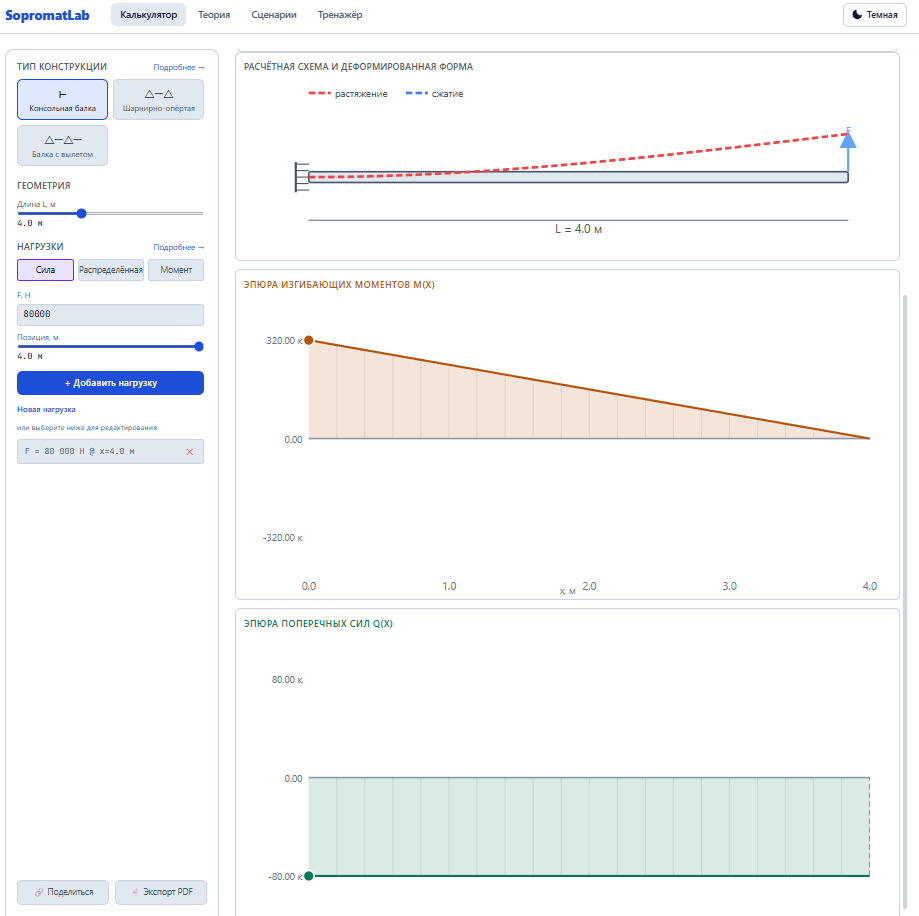
\includegraphics[width=0.75\textwidth]{images/cantilever_scheme.png}
  \caption{Расчётная схема консольной балки}\label{fig:cantilever_scheme}
\end{figure}

\textbf{Граничные условия:}
\begin{equation}
  v(0) = 0, \qquad \theta(0) = 0,
  \label{eq:cant_bc}
\end{equation}
где $v(x)$ --- прогиб, $\theta(x)$ --- угол поворота сечения.

\textbf{Вывод формул для реакций.} Рассмотрим равновесие отделённой балки как жёсткого тела. Уравнения равновесия в плоскости $xOy$ имеют вид: $\sum F_y = 0$ и $\sum M_{A} = 0$, где точка~$A$ --- место заделки ($x = 0$). Из первого уравнения (сумма вертикальных проекций) получаем $R_{\text{зад}} - \sum_i F_i = 0$, откуда следует формула для вертикальной реакции. Из второго уравнения (сумма моментов относительно заделки): $M_{\text{зад}} - \sum_i F_i \cdot a_i = 0$, что даёт формулу для реактивного момента.

\textbf{Реакции:}
\begin{equation}
  R_{\text{зад}} = \sum_{i} F_i, \qquad M_{\text{зад}} = \sum_{i} F_i \cdot a_i,
  \label{eq:cant_reactions}
\end{equation}
\begin{conditions}
  R_{\text{зад}} & вертикальная реакция заделки, \textit{Н}; \\
  M_{\text{зад}} & реактивный момент заделки, \textit{Н$\cdot$м}; \\
  F_i & $i$-я сосредоточенная сила, \textit{Н}; \\
  a_i & расстояние от заделки до точки приложения $F_i$, \textit{м}.
\end{conditions}

Консольная балка характерна тем, что максимальный изгибающий момент всегда возникает в заделке, а максимальный прогиб --- на свободном конце~\cite{feodosev}:
\begin{equation}
  v_{\max} = \frac{F \cdot L^3}{3 \, EI} \quad \text{(для сосредоточенной силы на конце)}.
  \label{eq:cant_vmax}
\end{equation}

\textbf{Типичный учебный сценарий:} расчёт шасси самолёта. Стойка шасси моделируется как консольная балка длиной $L = 1{,}2$~м, нагруженная силой $F = 80$~кН на свободном конце (сценарий~2 платформы).

\subsubsection{Шарнирно-опёртая балка}

Шарнирно-опёртая (двухопорная) балка --- балка на двух шарнирных (неподвижных) опорах~\cite{darkov}. Опора~$A$ расположена в точке $x = 0$, опора~$B$ --- в точке $x = L$. Расчётная схема показана на рис.~\ref{fig:ss_scheme}.

\begin{figure}[H]
  \centering
  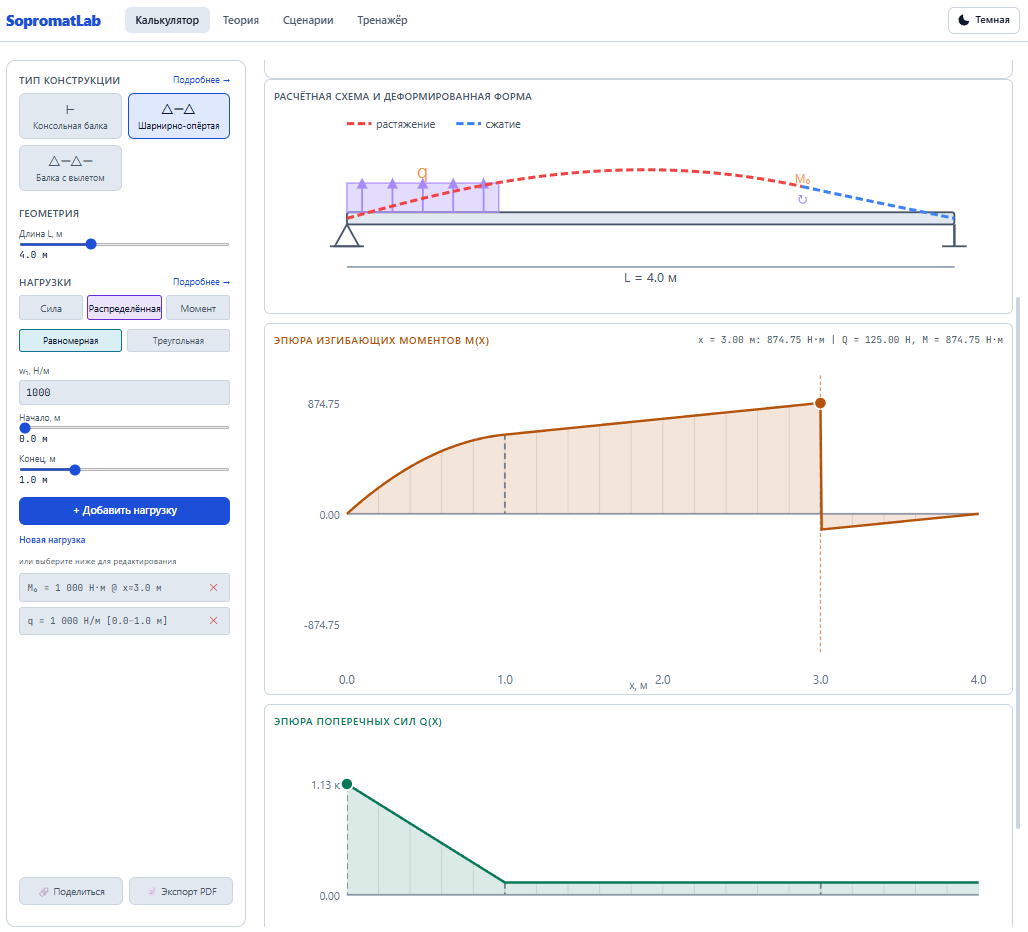
\includegraphics[width=0.75\textwidth]{images/simply_supported_scheme.png}
  \caption{Расчётная схема шарнирно-опёртой балки}\label{fig:ss_scheme}
\end{figure}

\textbf{Граничные условия:}
\begin{equation}
  v(0) = 0, \qquad v(L) = 0.
  \label{eq:ss_bc}
\end{equation}

\textbf{Вывод формул для реакций.} Для определения реакций запишем два уравнения равновесия: сумму проекций на ось $y$ и сумму моментов относительно опоры~$B$:
\[
  \sum F_y = R_A + R_B - \sum_i F_i = 0,
\]
\[
  \sum M_B = -R_A \cdot L + \sum_i F_i \cdot (L - a_i) = 0.
\]
Из второго уравнения непосредственно получаем выражение для реакции $R_A$; подставив его в первое уравнение, находим $R_B$. Полученные формулы имеют ясный физический смысл: реакция каждой опоры пропорциональна <<ближости>> нагрузки к противоположной опоре (правило рычага).

\textbf{Реакции:}
\begin{equation}
  R_A = \frac{\sum_i F_i \cdot (L - a_i)}{L}, \qquad R_B = \sum_i F_i - R_A.
  \label{eq:ss_reactions}
\end{equation}

Для шарнирно-опёртой балки характерно наличие экстремума изгибающего момента в сечении, где поперечная сила обращается в нуль: $Q(x_0) = 0 \Rightarrow M(x_0) = M_{\max}$~\cite{belyaev}. Максимальный прогиб при симметричном нагружении совпадает с серединой пролёта:
\begin{equation}
  v_{\max} = \frac{F \cdot L^3}{48 \, EI} \quad \text{(центральная сосредоточенная сила)}.
  \label{eq:ss_vmax}
\end{equation}

\textbf{Типичные учебные сценарии:}
\begin{itemize}
  \item Мостовой пролёт: балка длиной $L = 12$~м под двумя сосредоточенными силами $F_1 = 60$~кН ($a_1 = 3$~м) и $F_2 = 120$~кН ($a_2 = 7$~м) --- моделирует нагрузку от грузового автомобиля (сценарий~1).
  \item Ось тележки вагона: балка $L = 1{,}8$~м, две силы по $50$~кН и распределённая нагрузка $q = 8$~кН/м (сценарий~5).
\end{itemize}

\subsubsection{Балка с вылетом}

Балка с вылетом (консольным свесом) --- двухопорная балка, у которой один конец выступает за пределы опоры~\cite{aleksandrov}. Опора~$A$ расположена в точке $x = 0$, опора~$B$ --- в точке $x = L$, консольный вылет простирается от $x = L$ до $x = L + c$, где $c$ --- длина вылета. Расчётная схема балки с вылетом показана на рис.~\ref{fig:overhang_scheme}.

\begin{figure}[H]
  \centering
  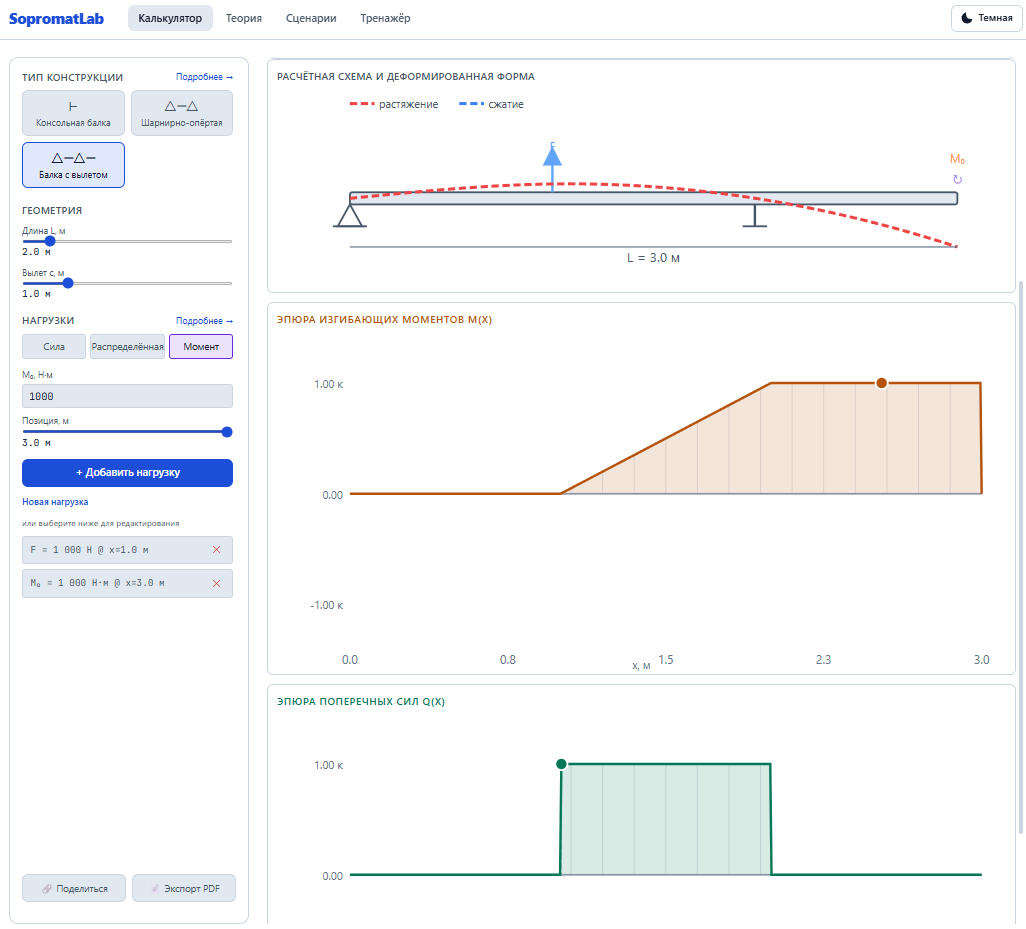
\includegraphics[width=0.8\textwidth]{images/overhang_scheme.png}
  \caption{Расчётная схема балки с вылетом}\label{fig:overhang_scheme}
\end{figure}

\textbf{Граничные условия:}
\begin{equation}
  v(0) = 0, \qquad v(L) = 0.
  \label{eq:oh_bc}
\end{equation}

\textbf{Реакции:}
\begin{equation}
  R_A = \frac{\sum_i F_i \cdot (L - a_i)}{L}, \qquad R_B = \sum_i F_i - R_A,
  \label{eq:oh_reactions}
\end{equation}
при этом координата $a_i$ может превышать $L$ для нагрузок, расположенных на вылете.

Особенности балки с вылетом~\cite{darkov, belyaev}:
\begin{itemize}
  \item Реакция $R_A$ может быть отрицательной, если преобладает нагрузка на вылете (опора <<прижимается>> вниз, балка стремится <<опрокинуться>>).
  \item Эпюра изгибающего момента меняет знак при переходе через опору~$B$, что создаёт перегиб деформированной оси.
  \item Над опорой~$B$ момент $M(L)$ отличен от нуля (в отличие от шарнирно-опёртой балки).
\end{itemize}

\textbf{Типичный учебный сценарий:} рельс под подвижной нагрузкой. Балка $L = 6$~м с вылетом $c = 1$~м, сосредоточенная сила $F = 100$~кН в точке $a = 3$~м (сценарий~3).

\subsubsection{Типы нагрузок}

Платформа поддерживает три типа внешних нагрузок, охватывающих все основные виды силового воздействия, рассматриваемые в учебных задачах~\cite{feodosev, stepin}.

\textbf{1. Сосредоточенная сила} (PointLoad) --- сила~$F$ (Н), приложенная в точке $x = a$. Вызывает скачок эпюры поперечной силы на величину $F$ и излом эпюры изгибающего момента:
\begin{equation}
  \Delta Q = F, \qquad \Delta M' = F.
  \label{eq:point_load_effect}
\end{equation}

\textbf{2. Распределённая нагрузка} (DistributedLoad) --- интенсивность $q(x)$ (Н/м), действующая на участке $[x_1, x_2]$. Реализованы два подтипа:
\begin{itemize}
  \item \textit{Равномерная нагрузка} --- постоянная интенсивность $q$ на участке:
  \begin{equation}
    F_{\text{рез}} = q \cdot (x_2 - x_1), \qquad x_c = \frac{x_1 + x_2}{2}.
    \label{eq:uniform_load}
  \end{equation}
  \item \textit{Треугольная нагрузка} --- линейно меняющаяся интенсивность от $q_1$ до $q_2$:
  \begin{equation}
    F_{\text{рез}} = \frac{q_1 + q_2}{2} \cdot l, \qquad
    x_c = x_1 + l \cdot \frac{q_1 + 2 q_2}{3(q_1 + q_2)},
    \label{eq:triangular_load}
  \end{equation}
  где $l = x_2 - x_1$ --- длина участка нагружения.
\end{itemize}

\textbf{3. Сосредоточенный момент} (MomentLoad) --- момент $M_0$ (Н$\cdot$м), приложенный в точке $x = a$. Вызывает скачок эпюры изгибающего момента на величину $M_0$, при этом эпюра поперечной силы не изменяется:
\begin{equation}
  \Delta M = M_0, \qquad \Delta Q = 0.
  \label{eq:moment_load_effect}
\end{equation}

\subsubsection{Область применимости расчётных случаев}

Рассматриваемые в работе типы балочных конструкций покрывают значительную часть инженерных задач базового курса сопротивления материалов. Область их применимости ограничена следующими условиями~\cite{feodosev, aleksandrov, belyaev}:

\textbf{1. Геометрические ограничения.} Соотношение длины пролёта к высоте поперечного сечения должно удовлетворять условию $L / h \geq 10$, что обеспечивает применимость теории тонких балок (гипотезы Бернулли). При меньших соотношениях необходимо учитывать влияние поперечных сдвигов по теории Тимошенко~\cite{timoshenko}.

\textbf{2. Ограничения на величину прогибов.} Прогибы должны быть малыми по сравнению с длиной балки: $v_{\max} / L < 1/200$~(для гражданских конструкций) или $< 1/300$~(для мостовых конструкций)~\cite{darkov}. При больших прогибах линейная теория становится неприменимой, и требуется учёт геометрической нелинейности.

\textbf{3. Линейно-упругий режим работы материала.} Напряжения в материале не должны превышать предел пропорциональности. Для конструкционной стали предел пропорциональности составляет около~$\sigma_{\text{пц}} \approx 200$~МПа, для алюминиевых сплавов~$\approx 150$~МПа, для древесины~$\approx 10$~МПа~\cite{gere2018}. При превышении этих значений возникают пластические деформации, и линейная теория становится неприменимой.

\textbf{4. Квазистатический характер нагружения.} Нагрузки считаются приложенными настолько медленно, что инерционные эффекты пренебрежимо малы. Платформа не рассчитана на динамические задачи (ударные нагрузки, свободные колебания, вибрации), которые требуют отдельной теории.

\textbf{5. Постоянство поперечного сечения.} Рассматриваются балки постоянного (призматического) сечения. Задачи с переменным сечением (например, балки с переменной шириной или со ступенчатым изменением высоты) могут быть сведены к разрабатываемой модели путём введения эффективного момента инерции, однако это требует дополнительной теоретической проработки.

Все перечисленные ограничения типичны для базового курса сопротивления материалов и не снижают учебной ценности платформы, поскольку соответствуют классу задач, изучаемых в первой части курса. Более сложные случаи (балки переменного сечения, динамические задачи, статически неопределимые системы, учёт сдвига) являются естественными направлениями развития работы.

\subsubsection{Сводная характеристика расчётных случаев}

Характеристики реализованных в платформе расчётных случаев сведены в таблицу~\ref{tab:cases}.

\begin{table}[H]
\caption{Сравнительная характеристика расчётных случаев}\label{tab:cases}
\small
\begin{tabularx}{\textwidth}{|>{\raggedright\arraybackslash}p{4.4cm}|>{\centering\arraybackslash}X|>{\centering\arraybackslash}X|>{\centering\arraybackslash}X|}
\hline
\textbf{Параметр} & \textbf{Консоль} & \textbf{Шарн.-оп.} & \textbf{С~вылетом} \\
\hline
Число опор & 1 (заделка) & 2 (шарниры) & 2 (шарниры) \\
\hline
Число реакций & 2 ($R_{\text{зад}}$, $M_{\text{зад}}$) & 2 ($R_A$, $R_B$) & 2 ($R_A$, $R_B$) \\
\hline
Статическая определимость & да & да & да \\
\hline
Граничные условия для $v$, $\theta$ & $v(0)\!=\!0$, $\theta(0)\!=\!0$ & $v(0)\!=\!0$, $v(L)\!=\!0$ & $v(0)\!=\!0$, $v(L)\!=\!0$ \\
\hline
Положение $M_{\max}$ & в заделке & где $Q=0$ & у опоры~$B$ или где $Q=0$ \\
\hline
Положение $v_{\max}$ & свободный конец & в пролёте & свободный конец вылета или в пролёте \\
\hline
Возможность $R_A < 0$ & --- & нет & да \\
\hline
Смена знака $M(x)$ & обычно нет & обычно нет & да (над опорой $B$) \\
\hline
\end{tabularx}
\end{table}

